\section{Synthesis of Tenant Policies} \label{sec:synthesisalgo}

The problem statement here is as follows: Given the network topology
graph and the set of tenant policies written in GPL, generate paths in
the network for every source-destination pair 
(derived from reachability policies)
satisfying all policies.  To achieve this, \Name
creates constraints that encode the forwarding and reachability rules
pertaining to the paths such that they satisfy the input policies.
The synthesized solution of paths obtained from the constraints are
then translated to switch forwarding rules.  
%To provide support for
%tenant policies in \Cref{tab:policysupport}, \name uses propositional
%logic (SAT) and linear rational arithmetic (LRA).

%% , and linear optimization
%% objectives for traffic engineering.

\subsection{Network Forwarding Model} \label{sec:fwdmodel}

We start by describing the basic forwarding model we use in \Name.
We define the physical switch topology as an undirected graph $T=(S, L)$,
where $S$ is the set of switches and $L$ is the set of links. 
We use the neighbour function $N(s) = \{s'\ | \ (s,s') \in L \}$ to denote 
the set of neighbour switches of $s$. 
We assume a set of packet classes $PC : [0,\lambda]$ 
and map each reachability policy to a unique integer in $PC$. In the rest of the paper, 
we often use the term packet class to identify the corresponding reachability policy. 
Other policies are not mapped to packet classes as they do not produce a path, but specify restrictions on paths of packet classes. 
We use $R$ to denote the set of reachability policies; each policy $r \in R$ is
a pair
$(predicate$:$src >> W_1;W_2; \ldots W_n >> dst, pc)$ where:
\begin{compactitemize}
\item  $predicate$ is the packet header identifier pertaining to $r$;
\item  $src,dst \in S$ are the source and destination switches;
\item $W_1, W_2, \ldots, W_n \subseteq S$ are the (potentially empty) ordered sets of waypoints; 
\item $pc \in PC$ is the packet class and is a unique integer used to identify the variables associated to $r$
\end{compactitemize} 
%Assuming that the intersection of predicates is empty for policies in $R$, we create a mapping $\gamma : R \rightarrow PC$ to associate each reachability policy with a unique integer called packet class in the set $PC$. Switches $src, dst \in S$ denote the ingress and egress switches respectively for the packet class $pc = \gamma(r)$ and Genesis finds a path from $src$ to $dst$ for $pc$. If a waypoint policy is specified, $W$ is the set of switches the path from $src$ to $dst$ must traverse through in no particular order.
We fix a constant $\mu$ and assume all paths to have length at most $\mu$. 
$K=[0,\mu]$ is the set of all permissible path lengths. The network forwarding
 model abstracts the actual forwarding rules at each node and encodes 
 the reachability of each packet class. 
 
We use the relation $Fwd \subseteq S \times S \times PC $  to capture 
the network forwarding behavior,---i.e. 
$(sw_1, sw_2$, $pc)\in$ $Fwd$ if 
$sw_1$ forwards packets of class $pc$ to switch $sw_2$. 
	We use the relation $Reach \subseteq S \times PC \times K$ to capture
	 the path reachability,---i.e. $(sw, pc, k)\in Reach$ if 
	the switch $sw$ is reachable in the path from the source
	 switch of packet class $pc$ in exactly $k$ steps.  
For brevity, we write $Fwd(sw_1, sw_2, pc)$ for $(sw_1, sw_2, pc) $ $\in Fwd$ and similarly for the $Reach$ relation. 
Since $Fwd$ depends on the topology,
for all $sw_1, sw_2$ that are not connected by a link, 
we have that $\forall pc$, $(sw_1,sw_2,pc) \notin Fwd$. 

Given a set of policies, \name generates a set of constraints
denoted by $\Psi$ over the $Fwd$ and $Reach$ relations. 
$(Fwd,Reach) \models \Psi$ denotes that 
$Fwd$ and $Reach$ is a model of $\Psi$.

\begin{mydef} \label{def:Pi}
Given two concrete relations $Fwd$ and $Reach$, 
the set of induced paths $\Pi = \texttt{paths}(Fwd, Reach)$ is defined as follows:
given a class $pc$,  $(sw_0 \ldots sw_k, pc) \in \Pi$ iff : 
\begin{compactenumerate}
	\item $\forall i \in [0,k]. (sw_i, pc, i) \in Reach$
	\item $\forall i \in [0, k - 1]. (sw_i, sw_{i+1}, pc) \in Fwd$
\end{compactenumerate}
\end{mydef}
\noindent Figure~\ref{fig:model} illustrates these definitions.

\begin{figure}
	\centering
	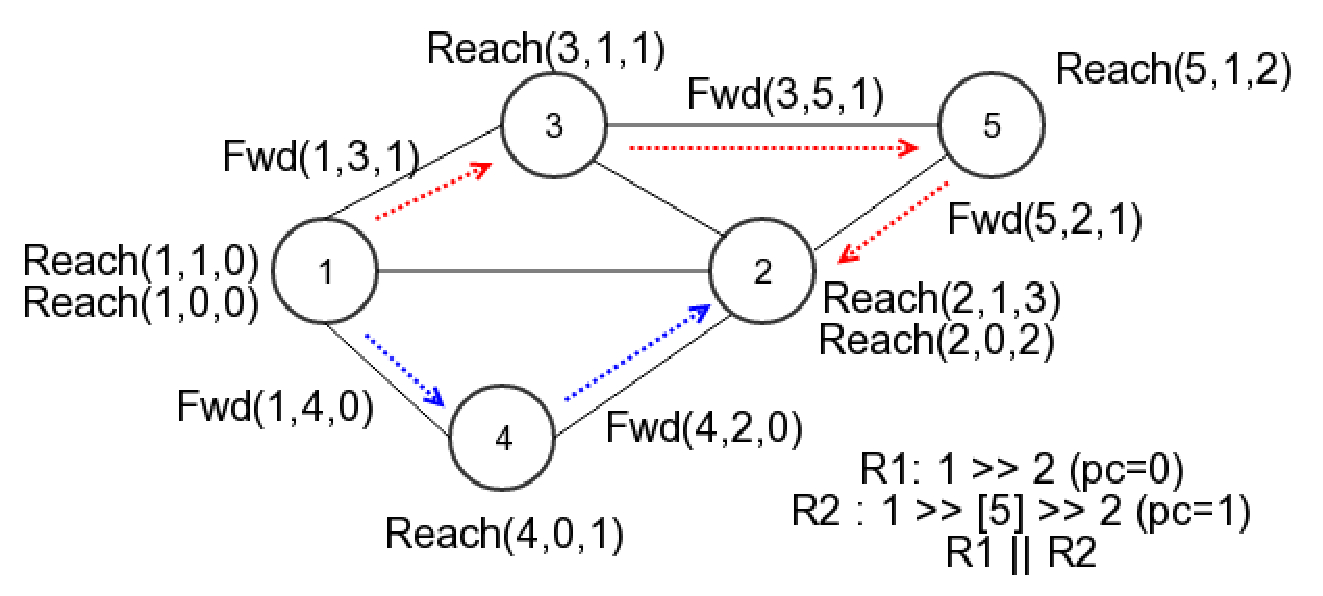
\includegraphics[width=0.8\columnwidth]{figures/network-model-example.eps}
	\caption{Values of the $Fwd$ and $Reach$ relations of the network forwarding model
		 for the policies specified in the figure. The blue and red arrows indicate the 
		 paths of packet classes 0 and 1 respectively according to the model.}
	\label{fig:model}
\end{figure}

\begin{mydef}
Given the set of constraints $\Psi$ corresponding to the input policies,
a set of paths $\Pi$ is a solution to $\Psi$, $\Pi \models \Psi$, 
if there exists $Fwd, Reach$ such that $(Fwd, Reach) \models \Psi$ and $\ \Pi=\texttt{paths}(Fwd,Reach)$.

\end{mydef}
%An example network forwarding model is shown in \cref{fig:model}. 
%%There are two reachability policies, $r1 : 1 >> [5] >> 2$ with $pc=1$ and $r2 : 1 >> 2$ with $pc=2$ and $r1$ is isolated to $r2$
%Using the value of $Fwd$ relation, we can find out paths for each packet class the forwarding rules for each switch. 

In practice, we  
model the forwarding and reachability relations using propositions and
 reduce enforcement of tenant policies like reachability, waypoints 
 and isolation to a Boolean Satisfiability Problem (SAT) problem\footnote{
 	An earlier iteration of our model used \emph{uninterpreted functions} 
 	and modeled reachability using recursive constraints, 
	which was slower with a greater number of constraints.}. 
Using these
relations, operators can write custom policies in a concise and intuitive
manner. 

\subsection{Reachability} \label{sec:reach}
We first discuss the constraints added to $\Psi$
for reachability policies without waypoints.
For a reachability policy $s >> d$ and packet class $pc$, the added constraints must ensure that 
the solution model represents a path 
from source to destination. 
The base constraint states that $(s, pc,0) \in Reach$ meaning
that $s$ can be reached in $0$ steps. 
The following constraint states that there must be a forwarding rule from $s$ to one of
the neighbors of $s$\footnote{
	We unroll the existential quantifier $\exists n \in N(s)$ using disjunction of 
	clauses $\bigvee\limits_{n \in N(s)}$ and
	the universal quantifier $\forall n \in N(dst)$ using conjunction of clauses $\bigwedge\limits_{n \in N(dst)}$
	and stay in propositional logic.}.
\begin{equation} \label{eq:src}
	\exists n \in N(s).~Fwd(s, n, pc) \wedge Reach(n, pc, 1).
\end{equation}
Next, we add the following constraints that state that $d$ can be reached in some number of steps and,
since $d$ is the last switch in the path, there are no forwarding rules from it.
\begin{equation} \label{eq:dst}
	\exists k.~Reach(d, pc, k) \ \wedge \ \forall n \in N(d). \ \neg Fwd(d, n, pc).
\end{equation}
Finally, we add implication constraints that propagate reachability backward from destination to source. 
If a node $n_1$ is reachable in $k$ steps, there must be a node $n_2$ reachable in  $k-1$ steps and 
a forwarding rule $n_2 \rightarrow n_1$.
\begin{multline} \label{eq:bckprop}
\forall n_1,k.~ Reach(n_1,pc,k) \implies \exists n_2.  n_2 \in N(n_1) \wedge \\ Reach(n_2,pc,k-1) \wedge Fwd(n_2,n_1,pc).
\end{multline} 
When combined together, these constraints %can only be satisfied if there is a valid path from $s$ to $d$.
% to destination by using the unit clauses in \cref{eq:dst}, and finding a path from destination back to a switch $sw$ which is a neighbour of $src$. $Reach(sw,pc,1)$ would be true from \cref{eq:src} and the reachability policy would be satisfied. 
are sufficient to ensure the existence of a path from $s$ to $d$ for packet class $pc$.
% in terms of the forwarding relation $Fwd$. 
However, since there is no restriction on the number of $Fwd$ values that can be true at a switch, we can get multiple forwarding rules at switches, and 
also multiple paths to the destination. 
These can also create forwarding loops. 
Concretely, this is not a problem: as long as there is  at least one path from $s$ to $d$ we can recover it from the solution of the constraints. 
Moreover, this representation is quite efficient, as forcing a single path would
require adding further constraints (\secref{sec:waypoint}) and increase the synthesis
time.
% we are able to extract a path from the solution without 
%adding additional constraints to ensure the semantics of \emph{unicast} forwarding. 

To extract a concrete $s$-to-$d$ path we 
perform a breadth-first search on the reachability graph induced by the solution to the constraints. 
A directed edge $n_1 \rightarrow n_2$ appears in the reachability-graph if there is a 
forwarding rule indicated by the relation $(n_1,n_2, pc) \in Fwd$. 
We extract the rules relevant to the shortest path from source to destination from the model, and the additional rules obtained in the solution (extra paths, forwarding loops) are ignored.  

\subsection{Waypoint Traversal} \label{sec:waypoint}
For a reachability policy with a sequence of waypoint sets $s >> W_1;\ldots;W_n >> d$ and packet class $pc$, we add all the constraints specified in \secref{sec:reach} to ensure the existence of a path from $s$ to $d$. We then add constraints so that all waypoints $w$
are traversed. 
\begin{equation} \label{eq:waypoints}
	\forall w \in W_1, \ldots, W_n. \ \exists k.~Reach(w, pc, k).
\end{equation}
For each set $W_i$ for $i>1$, we add constraints to ensure that all waypoints
in $W_i$ are reached after all waypoints in $W_{i - 1}$ : 
\begin{multline}
\forall w_{i} \in W_{i}, \forall k_i.~Reach(w_i, pc, k_i) \implies 
\forall w_{i - 1} \in W_{i-1}. \\ \exists k_{i-1}. \ 
 k_{i-1} < k_{i} \wedge Reach(w_{i-1}, pc, k_{i-1}).
\end{multline}
%TODO
Previously, we imposed no restriction on the number of paths 
from $s$ to $d$. In the case of waypoints, this can result in 
a solution with multiple paths, with each individual path traversing
some of the waypoints, which is not the correct enforcement for a waypoint policy.
Thus, we need to ensure the solver returns a single path traversing
all the waypoints. To achieve this, we limit the number of
forwarding rules for $pc$ at a switch to 0 or 1. 
%%However, just ensuring reachability of waypoints is not sufficient. Since, we do not have any restrictions on the count of forwarding rules for a packet class at a switch, it is possible that waypoints are reachable from the source through separate paths, and do not lie in the path from source to destination. Thus, to ensure that all waypoints are reachable in the path from source to destination, we need to add constraints on the count of forwarding rules at each switch. 
%Forwarding rule constraints are to ensure that the forwarding relation $Fwd$ for a switch contains a \emph{single} switch which is a \emph{neighbour} or to no node at all (switches which are not reached in the path, and the destination will not have any forwarding rules). 
We define the forwarding set as:
\begin{equation}
	FwdSet(sw,pc) = \{k \ | \ Fwd(sw,k,pc)\}.
\end{equation}
We then add constraints stating that the size of the forwarding set must not exceed 1:
\begin{equation}
		\forall sw,pc .\ |FwdSet(sw,pc)| \leq 1 \label{eq:fwdset}.
\end{equation}
Here $|A|$ denotes the size of set $A$. The above constraints are expressed in SAT 
as follows: 
\begin{equation}
\bigvee_{\mathclap{k_1 \in N(sw)}} Fwd(sw, k_1, pc) \wedge (\bigwedge_{\mathclap{k_2 \in N(sw), k_2 \not= k_1}} \neg Fwd(sw, k_2, pc))
\end{equation}
%The forwarding set constraints ensure that the forwarding rules exist only on the path from source to destination, and no other rules exist in the solution. If a switch has a forwarding rule to  elsewhere, then it would not have a rule for the path, and the destination will not be reachable. These restrictions will also ensure there are no forwarding loops in the path. 
Since, there cannot exist multiple rules at a switch, the model will contain a 
single path from source to destination for $pc$ traversing the
waypoints in the right order.
%There would have to 
%be more than one rule at a switch for multiple paths from the source to exist. 

\subsection{Isolation}
A traffic isolation policy $pc_1 || \ pc_2$ states that the paths for
$pc_1$ and $pc_2$ do not share any link in the same direction.  We
enforce this policy by adding to $\Psi$, constraints stating that at every
switch, $pc_1$ and $pc_2$ must not forward to the same switch:
\begin{equation}
	\forall n_1.~\neg ( \exists n_2. Fwd(n_1,n_2,pc_1) \wedge Fwd(n_1,n_2,pc_2)). \label{eq:isolation}
\end{equation}
For a link isolation policy $pc_1 <> \ pc_2$ which prevents sharing a link
in both directions, we add the constraints:
\begin{multline}
\forall n_1.~\neg ( \exists n_2. Fwd(n_1,n_2,pc_1) ~~\wedge \\ (Fwd(n_1,n_2,pc_2) \vee Fwd(n_2,n_1,pc_2))). \label{eq:linkisolation}
\end{multline}
%These constraints are sufficient to ensure that the packet classes $pc_1$ and $pc_2$ would be isolated. 
%When combined with \Cref{eq:fwdset}, these constraints guarantee
%isolation
%as there exists a single path for $pc_1$ and
%$pc_2$ which would be isolated. 
With single paths for $pc_1$ and $pc_2$ (when combined 
with \Cref{eq:fwdset}), the above constraints ensure those
paths are isolated. 
Interestingly, for a reachability policy without waypoints,  
the constraints in \Cref{eq:fwdset} are not required to enforce isolation. 
Even though the solver could produce multiple forwarding rules which induce multiple paths, 
the constraints in \Cref{eq:isolation} or \Cref{eq:linkisolation} guarantee 
isolation as the solver would discard
the rules conflicting with another packet class.

%reachability policy. Thus, the solver would remove the additional rules which conflict with
%the other class while still ensuring a path exists from source to destination. 

%The isolation constraints is intuitive when coupled with the forwarding set constraints (\cref{eq:fwdset}) as the model only has forwarding rules for the path from source to destination. However, for a reachability policy without waypoints, we argue that the forwarding set constraints are not required when coupled with the isolation constraints. The reasoning behind this is that the solver would simply remove the extra forwarding rules of a packet class in the model which conflict with the other packet class, as there are no constraints which require the need of these extra forwarding rules for correctness, but are one particular solution model in the space of solutions. 


%In terms of our model, the link capacity policy translates to constraints that
%ensure that the tuples of the form $(sw_1, sw_2, pc) \in Fwd$ for $pc \in PC$ conform to the capacity specified in the policy, 
%as the forwarding rule $sw_1 \rightarrow sw_2$ means that the link is being used by the particular packet class.
% 
%Let $C(sw_1,sw_2,pc)$ be the cumulative capacity function of the link used by all packet classes less than equal to $pc$. Since we use integers for denoting the packet class, we have a total order of the set of packet classes. We use this to create inductive constraints to sum over the set of Boolean variables $Fwd(sw_1, sw_2,pc)$. Let $PC : [0, \lambda]$ be the set of packet classes and $W(pc)$ 
%denote the capacity of packet class $pc$--i.e., the bandwidth allotted to the packet class. 
%The base case constraint for the capacity function is for $pc = 0$:
%\begin{multline}
%\neg Fwd(sw_1, sw_2, 0) \implies C(sw_1, sw_2, 0) = 0 \\
%	Fwd(sw_1, sw_2, 0) \implies C(sw_1, sw_2, 0) = W(0)
%\end{multline} 
%If link is used, the inductive constraints for the capacity function are as follows:
%\begin{multline}
%	\forall pc > 0.~Fwd(sw_1,sw_2,pc) \implies \\ C(sw_1, sw_2, pc) =  C(sw_1, sw_2, pc - 1) + W(pc)
%\end{multline}
%If the link is not used, the constraints are as follows : 
%\begin{multline}
%\forall pc > 0.~\neg Fwd(sw_1,sw_2,pc) \implies \\ C(sw_1, sw_2, pc) =  C(sw_1, sw_2, pc - 1)
%\end{multline}
%To satisfy the policy, the total capacity used should not exceed $\omega$. 
%Since $\lambda$ is the greatest element in $PC$ we have:
%\begin{equation}
%	C(sw_1, sw_2, \lambda) \leq \omega
%\end{equation} 
%For \emph{switch table size} policies, we need to track the number of packet classes that traverses the switch.
%We create inductive constraints similar to those for link capacity.
%. for counting the packet classes traversing $sw$.
